\section{Der Abtastsatz}

\begin{definition}\leavevmode
\begin{enumerate}
\item Eine Funktion $ f \in L_{1}(\R) $ heißt \emph{bandbeschränkt} mit \emph{Bandbreite $ t $} oder
  kurz \emph{$ T $-bandbeschränkt}, wenn
  \[
    \widehat{f}(\xi) = 0, \qquad \xi \notin [-T,T].
  \]
  Oder anders formuliert: Eine Funktion $ f \in L_{1}(\R) $ ist bandbeschränkt, wenn $ \widehat{f} $
  endlichen Träger besitzt.
\item Der \emph{Sinus Cardinalis} oder $ \sinc $-Funktion ist definiert als
  \[
    \sinc(x) \coloneqq \begin{cases}
      \frac{\sin(\pi x)}{\pi x}, & x \in \R \setminus \{ 0 \}, \\
      1, & x = 0.
    \end{cases}
  \]
\end{enumerate}
\end{definition}

\begin{remark}[Bandbeschränktheit]
Ist eine Funktion $ T $-bandbeschränkt, dann ist sie auch gleichzeitig $ T + n $-bandbeschränkt für
jedes $ n > 0 $.
\end{remark}

\begin{remark}[Sinus Cardinalis]\leavevmode
\begin{itemize}
\item Der Name stammt daher, dass die Funktion an allen ganzzahligen Stellen entweder den Wert 
  $ 0 $ oder $ 1 $ annimmt. Abbildung~\ref{fig:sinc} zeigt den Verlauf der $ \sinc $-Funktion.
  \begin{figure}[ht]
  \centering
  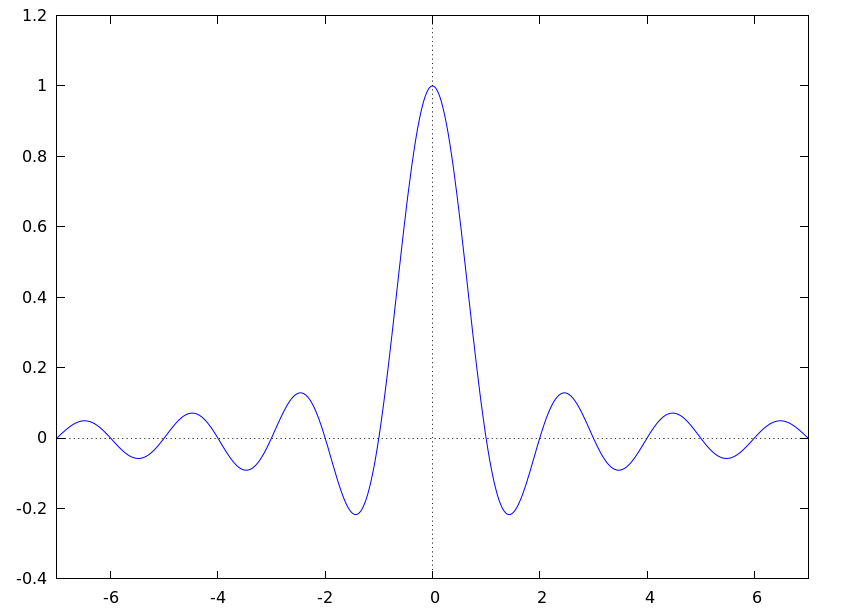
\includegraphics[width=0.7\textwidth]{Bilder/sinc}
  \caption{Plot der $ \sinc $-Funktion auf dem Intervall $ [-7,7] $.}
  \label{fig:sinc}
  \end{figure}
\item Fun fact: Es gilt
  \[
    \int_{\R} \sinc(x) \dif x = 1 \quad \text{und damit} \quad
    \int_{\R} \sinc(x / \pi) \dif x = \pi.
  \]
\item Die $ \sinc $-Funktion ist i.W.\ bis auf Normierung die Fourier-Transformierte der
  Rechtecksfunktion. Damit ist der $ \sinc $ der ideale Tiefpassfilter (aus Sicht des
  Frequenzbereichs).
\item Es kann aber gezeigt werden, dass $ \sinc \notin L_{1}(\R) $, weswegen der ideale 
  Tiefpassfilter nur näherungsweise implementiert werden kann. Es gilt aber
  $ \sinc \in L_{2}(\R) $, was u.a.\ ein Grund dafür ist, die Fourier-Transformation auf dem
  $ L_{2}(\R) $ einzuführen. Für Beweis siehe Anhang~\ref{sec:sincproofs}.
\end{itemize}
\end{remark}

\begin{proposition}[Abtastsatz von Shannon]
Ist $ f \in L_{1}(\R) $ eine $ T $-bandbeschränkte Funktion und ist $ h < \pi / T $, dann ist
\[
  f(x) = \left( (S_{h} \ f) * \sinc \right) \left( \frac{x}{h} \right) 
       = \sum_{k \in \Z} f(hk) 
           \frac{\sin \left( \pi \left( \frac{x}{h} - k \right) \right)}
                {\pi \left( \frac{x}{h} - k \right)}.
\]
\end{proposition}